\begin{tikzpicture}[x=0.142mm,y=-0.142mm]
  \node[anchor=north west,inner sep=0] at (0,0) {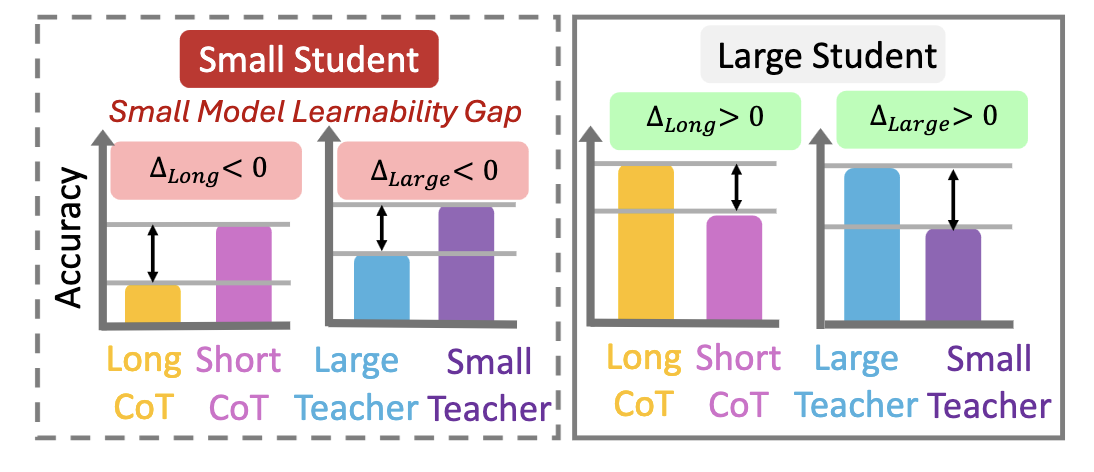
\includegraphics[width=155.348mm]{part6/visuals/student_learner.png}};
  \fill[red!80!black,rounded corners=3pt] (181,32) rectangle (437,87);
  \node[text=white,font=\small\bfseries] at (309,59) {小型学生模型};
  \fill[white] (106,94) rectangle (538,123);
  \fill[white] (106,121) rectangle (317,133);
  \fill[white] (340,121) rectangle (538,133);
  \node[text=red!80!black,font=\small] at (323,111) {小模型可学习性鸿沟};
  \fill[white] (48,159) rectangle (89,313);
  \node[rotate=90,font=\small\bfseries] at (68,237) {准确率};
  \fill[gray!10,rounded corners=3pt] (702,29) rectangle (945,81);
  \node[font=\small\bfseries] at (824,55) {大型学生模型};
  \fill[white] (97,335) rectangle (553,431);
  \fill[white] (599,335) rectangle (1057,431);
  \node[text=orange!90!yellow,align=center,font=\small] at (147,379) {长\\思维链};
  \node[text=magenta!55,align=center,font=\small] at (240,379) {短\\思维链};
  \node[text=cyan!75!blue,align=center,font=\small] at (364,379) {大型\\教师模型};
  \node[text=violet!85!black,align=center,font=\small] at (488,379) {小型\\教师模型};
  \node[text=orange!90!yellow,align=center,font=\small] at (644,379) {长\\思维链};
  \node[text=magenta!55,align=center,font=\small] at (739,379) {短\\思维链};
  \node[text=cyan!75!blue,align=center,font=\small] at (866,379) {大型\\教师模型};
  \node[text=violet!85!black,align=center,font=\small] at (988,379) {小型\\教师模型};
\end{tikzpicture}
